\chapter{Clustering}

\section{Previous Work}

PUT DISCUSSION OF OTHER CLUSTERING HERE [CLUSTERING OF OTHER COLLECTIONS OF GALAXIES, VARIOUS RANGES, LOOK AT HiCKOX et al. 2011-2012]

Previous work on clustering has been looked at different subpopulations of galaxies. 

\section{Method}

To compute the clustering and halo mass, a few steps must be done. 

\subsection{Autocorrelation Function}

The clustering is computed through a two point correlation function. The first step s to calculate the angular correlation function $ \omega(\theta)$. Once $ \omega(\theta)$ is computed, the second step is to obtain the two-point correlation function parameters of $r_0$ and $\gamma$.

The two-point correlation function is the the probability above Poisson of finding a galaxy in a volume element $dV$ at a physical separation $r$ from another randomly chosen galaxy, such that $$ dP = n[1 + \Eta(r)]dV$$, [REWORD] where $n$ is the mean space density of the galaxies in the sample. The estimator comes from Landy \& Szalay (1993) where $$ \omega(\theta) = \frac{1}{RR}(DD-2DR + RR)$$, there $DD$, $DR$, and $RR$ are the number of data-data, data-random, and random-random galaxy pairs at a separation $\theta$, where each of the three collections is normalized to sum to 1. 

Once the angular correlation function is found, a power-law model is fitted following $$\omega(\theta) = A\theta^{-\beta} $$

In this report, $\beta$ = 0.8, a value found for many other galaxy autocorrelations [CITE]. To convert the $A$ and $\beta$ to real-space $r_0$ and $\gamma$, the conversion can be found through the two equations

$$ \gamma = \beta + 1 $$ $$ A = H_{\gamma}\frac{\int_{0}^{\inf} (dN_1/dz)(dN_2/dz)E_z\chi^{1 - \gamma} dz}{[\int_{0}^{\inf} (dN_1/dz)dz][\int_{0}^{\inf} (dN_2/dz)dz]}r_0^{\gamma}$$

where $H_{\gamma} = \Gamma(0.5)\Gamma(0.5[\gamma -1])\Gamma(0.5\gamma)$, where $\Gamma$ is the gamma function, $\chi$ is the radial comoving distance, $dN_{1,2}/dz$ are the redshift distributions of the samples, where in the case of autocorrelation, are equal to each other, and $E_z = H_z/c = dz/d\chi$ \cite{hickox2011clustering}. The Hubble parameter $H_z$ can be found from
$$H_z^2 = H_0^2[\Omega_m(1+z)^3 + \Omega_{\lambda}]$$ \cite{hickox2011clustering}.

For this analysis, all CO line candidates above the 0.6 fidelity threshold were used, resulting in 35 sources, shown in Fig. \ref{fig:Clustering_points}. As a comparison, the two point correlation function was also computed for other fidelity cuts. The redshift distribution was taken from the CO redshifts of the lines, and the calculations were calculated over the range z = 1.5 to 3.5, as this is where the majority of the CO lines' redshifts are. Results over the range of z = 0 to z = 4.4 are also shown. 

\begin{figure}[tbp]
\centering 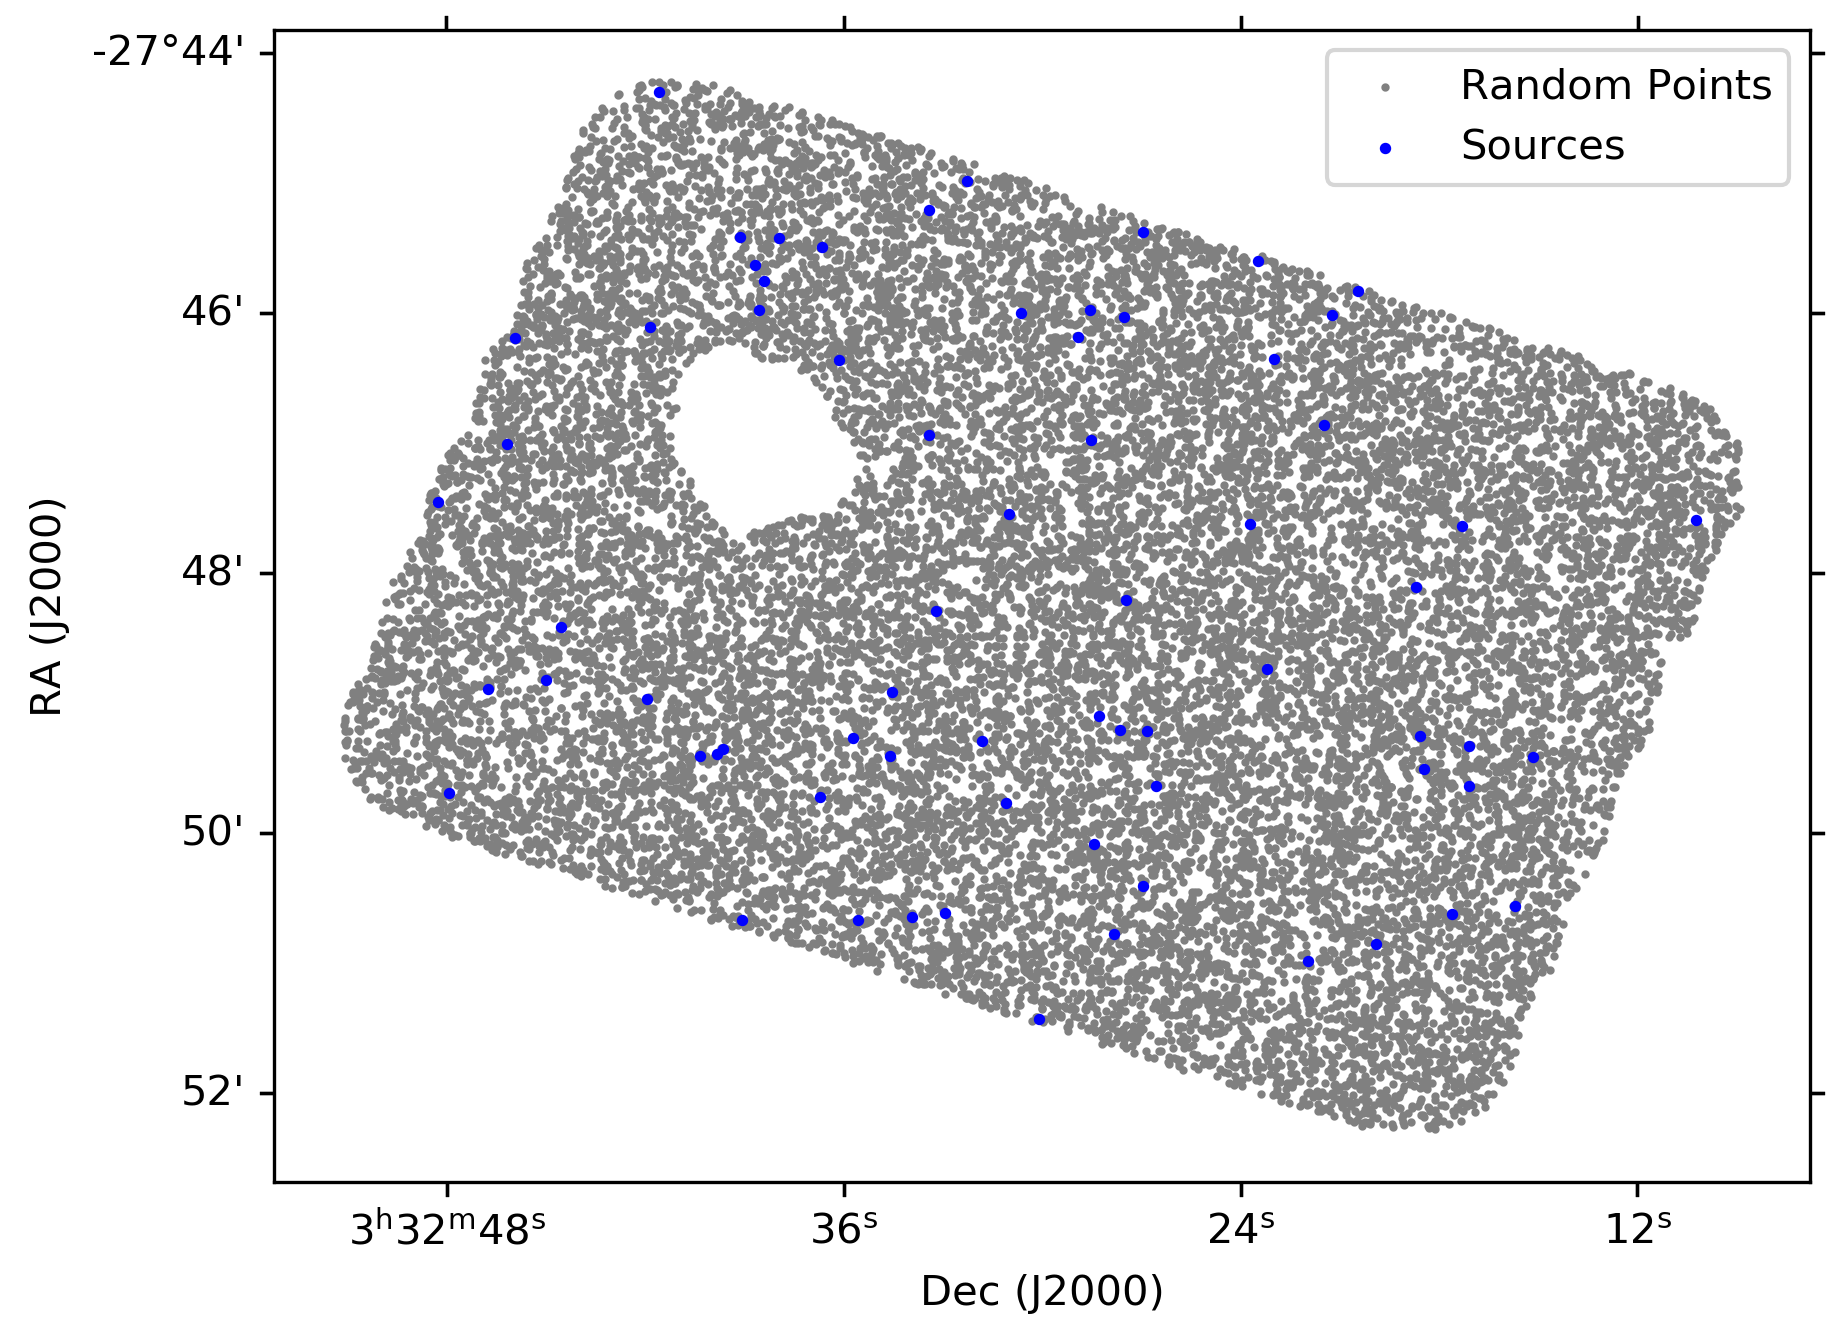
\includegraphics[width=120mm]{PDFS/NX_V_Y_Sources_20000.png}
\caption{Random points and sources from the $>$ 0.6 fidelity cut. The random points are distributed uniformly throughout the Wide ASPECS footprint.}
\label{fig:Clustering_points}
\end{figure}

\subsection{Halo Mass Calculation}

To determine the halo mass from the calculations[INCLUDE HALO MASS CALCULATIONS]

\cite{hickox2011clustering} used the HALOFIT code of Smith et al. 2003, to dtermine the non-linear power spectrum $\Delta_{NL}^2(k,z)$ of dark matter, assuming the cosmology and the slope of the initial fluctuation power spectrum $\Gamma = \Omega_mh = 0.21$. The Fourier transform of the nonlinear-dimensionless power spectrum gives the real-sapce correlation function $\Eta(r)$, which is then integrated to $\pi = 100 h^{-1} Mpc$ following Equation [INSERT] to obtain the dar kmatter projected correlation function $\omega^{DM}_p(R,z)$.

To obtain $\omega(\theta)$ for the dark matter, Limber's equation is used to project the power spectrum into the angular correlation. Specifically a Monte Carlo integration of Equation (A6) in Myers et al. 2007 is used to obtain $\omega(\theta)$ for dark matter. For each angular correlation analysis, we compute the average ration between the best-fit power law model and the dark matter $\omega(\theta)$ on scales from 8 arcminutes to 50 arcminutes, where $\omega(\theta$ is dominated by the two-halo term. This ratio gives us $b^2_{CO}$ for the CO autocorrelations. 

Finally, using $b^2_{CO}$ to estimate the charactersitic mass of the dark matter halos hosting each subset of 

\cite{hickox2011clustering} showed that for SMG galaxies, around a redshift of 2, the autocorrelation length $r_0 \approx 6 h^{-1} Mpc$. 

\section{Results}

As can be seen in Fig. \ref{fig:Angular_correlation}, as the fidelity increases, $A$ increases as well. When converted to $r_0$, the fidelity cuts result in $r_0$ values of 23 +- 5 for fidelity $>$ 0.7, 20 +- 2 for fidelity $>$ 0.6, 8 +- 1.5 for fidelity $>$ 0.5, and no $r_0$ for fidelity > 0.4, as the $A$ value is consistent with 0. 

\begin{figure}[tbp]
\centering 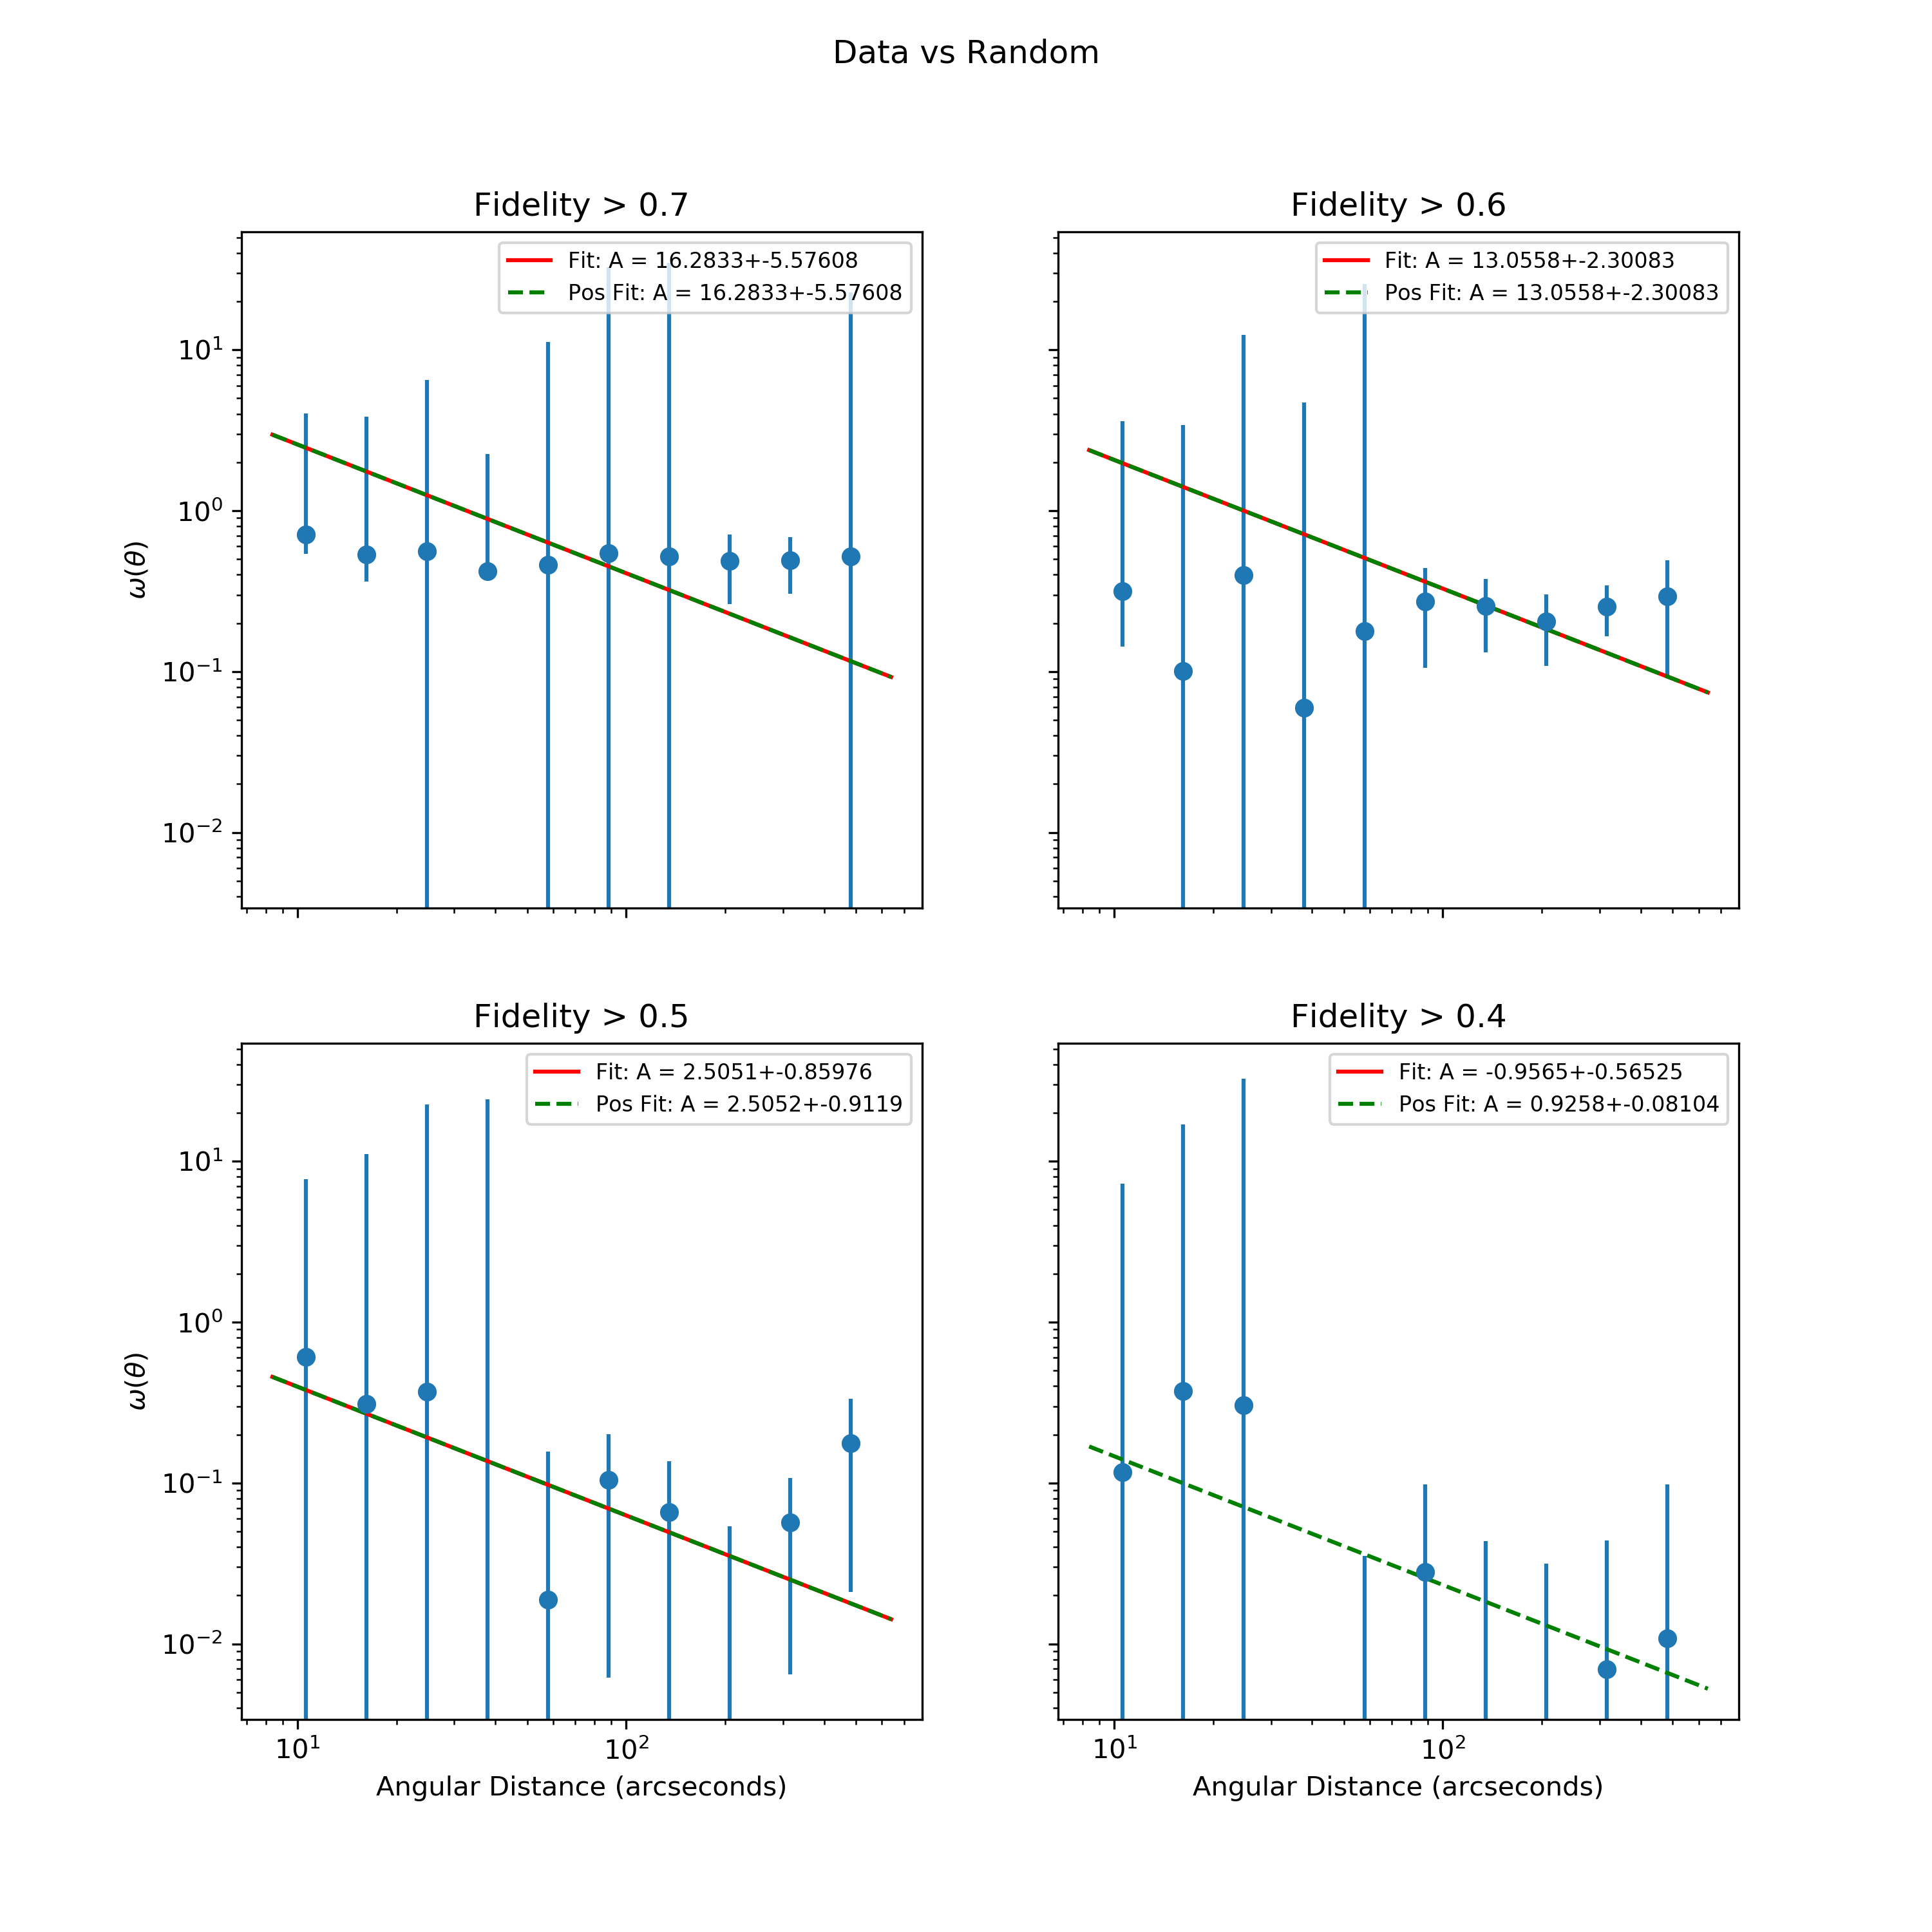
\includegraphics[width=120mm]{Fidelity/Log_4Panel_Data_Vs_Random_bin10_NFalse_Num10000.png}
\caption{Angular correlation function for various fidelity cuts. The red lines are from fitting $\omega(\theta) = A\theta^{-0.8} $ to all of the bins. The green dashed line is from fitting that same equation only to bins that had a positive value. As the fidelity goes up, the $A$ value increases as well, indicating stronger clustering, as is expected.}
\label{fig:Angular_correlation}
\end{figure}

Besides the different fidelity cuts, different binnings also are included to study their effects on the final $r_0$ results. 

\begin{figure}[tbp]
\centering 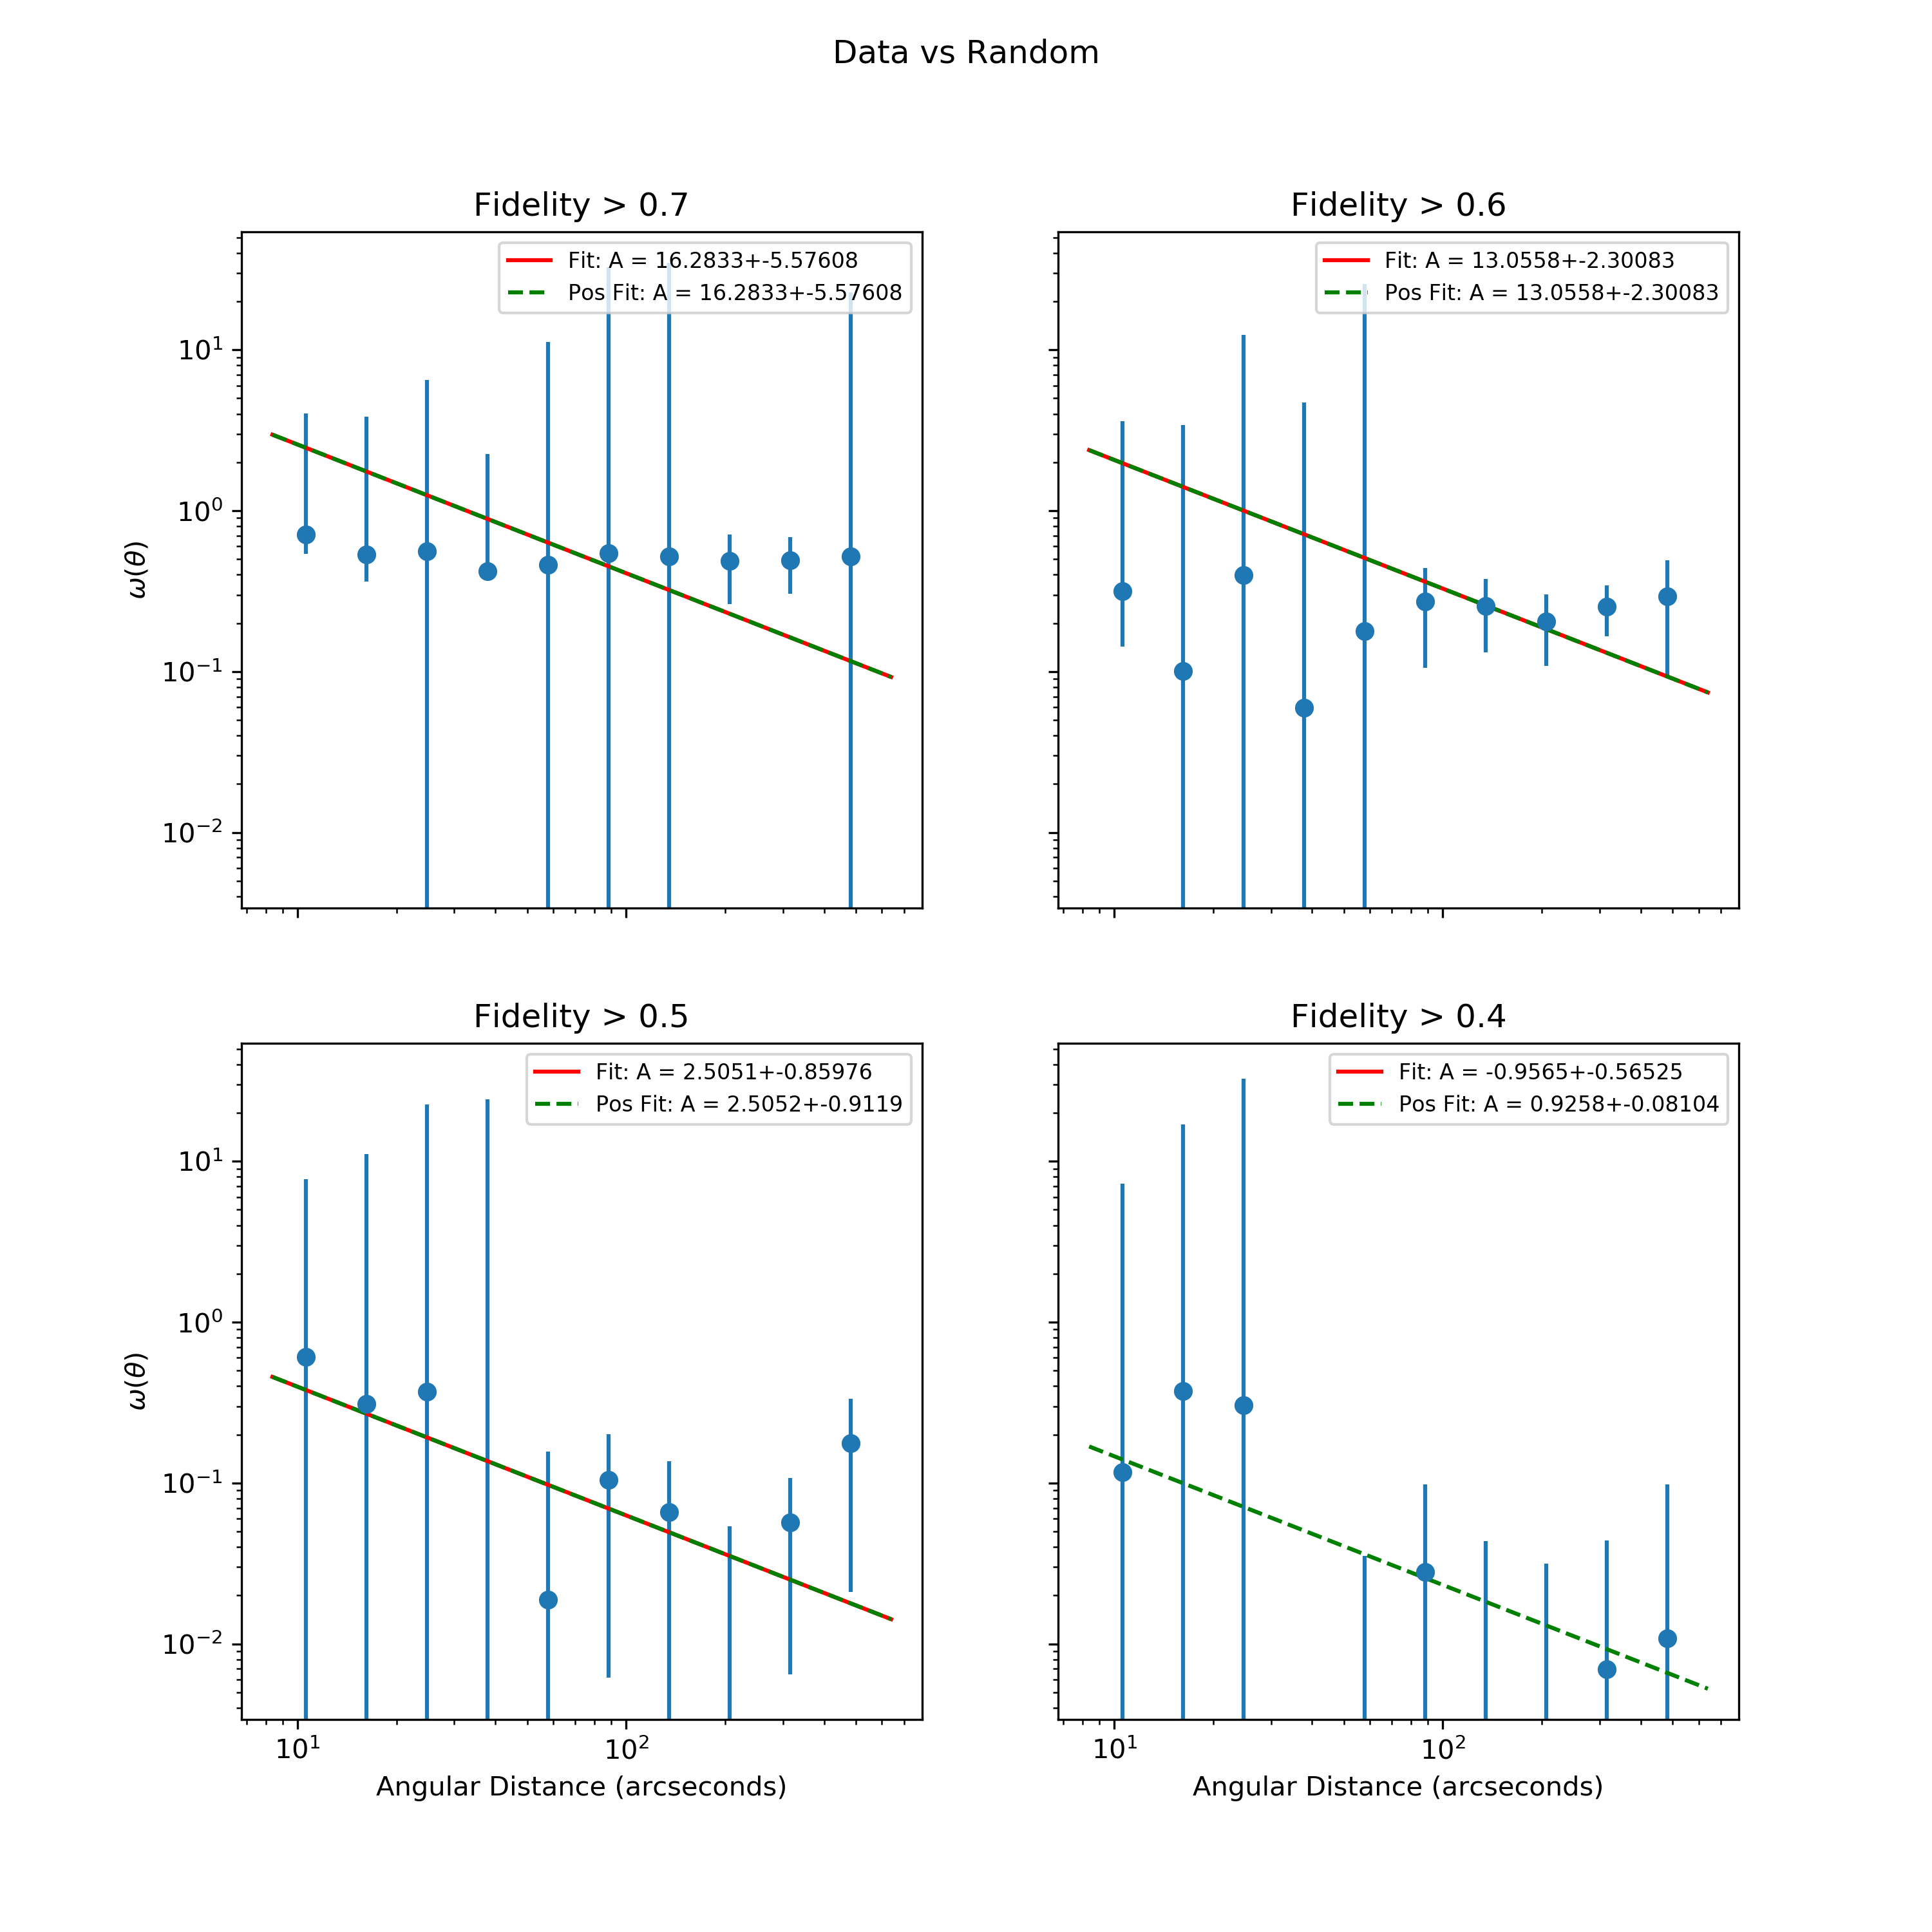
\includegraphics[width=120mm]{Fidelity/Log_4Panel_Data_Vs_Random_bin10_NFalse_Num10000.png}
\caption{Angular correlation function for various binnings.}
\label{fig:Angular_binnings}
\end{figure}

As should be expected, as the fidelity cut goes up, meaning a larger portion of the CO lines remaining are true sources, the clustering value becomes larger as well. Once the fidelity drops below 0.5, such that the majority of the lines should be false positives, the clustering values drop to be consistent with 0. The clustering values for a variety of fidelity cuts are shown in Table \ref{table:Clsutering}

[INCLUDE CLUSTERING TABLE HERE WITH RESULTS, A, r0, errors on both, number of sources used in each] \label{table:Clustering}

[INCLUDE PLOT OF DIFFERENT R0 VALUES DEPENDENT ON CLUSTERING -> HOW THAT AFFECTS THE VALUES]

[INCLUDE REDSHIFT DISTRIBUTION PLOT]

[TALK ABOUT DIFFERENCES BETWEEN LINEAR AND GAUSSIAN SENSETIVITY]

\section{Discussion}

The clustering results do show that there is a larger $r_0$ as the fidelity cut becomes higher, suggesting that there are real sources in the sample. On the other hand, the clustering measurement is still very noisy and future work will be required to get a better final clustering measurement. 

In comparison to other clustering measurements, \cite{hickox2011clustering} found an $r_0$ for quasers to be between 5.5 and 